\documentclass[12pt]{article}

% Packages

\usepackage[utf8]{inputenc}     % Кодировка utf8
\usepackage[russian]{babel}     % Языки: русский
\usepackage{amssymb,amsmath}    % Математические дополнения от AMS
\usepackage{cmap}               % Улучшенный поиск русских слов в полученном pdf-файле
\usepackage{listings}
\textheight=24cm                % Высота текста
\textwidth=16cm                 % Ширина текста
\oddsidemargin=0pt              % Отступ от левого края
\topmargin=-1.5cm               % Отступ от верхнего края
\parindent=0pt                  % Абзацный отступ
\parskip=0pt                    % Интервал между абзацами
\tolerance=2000                 % Терпимость к "жидким" строкам
\flushbottom                    % Выравнивание высоты страниц

\lstset{ %
language=Python
}

\usepackage{color}
\usepackage{url}
\usepackage{graphicx}
\usepackage[colorlinks,unicode]{hyperref}

\title{Отчет по заданию №1 Практикума на ЭВМ}
\author{Никишин Евгений, 317 группа}
\date{09.10.2015}

\begin{document}
\maketitle

\tableofcontents

\section{Введение}

Данное задание направлено на освоение языка Python и системы научных вычислений NumPy. Задание состоит из 8 задач, при этом для каждой из них нужно написать векторизованный, невекторизованный варианты, а также третий вариант на усмотрение студента. Затем предлагается исследовать скорости работы написанных алгоритмов и, для некоторых задач, сравнить с готовыми реализациями в библиотеке SciPy

\section{Задачи}
\subsection{Задача 1}

\subsubsection*{Формулировка}

Подсчитать произведение ненулевых элементов элементов на диагонали произвольной матрицы.

\subsubsection*{Описание решений}

1. Векторизованный
\begin{lstlisting}
def diag_nonzero_prod1(X):
    diag = np.diag(X)
    return np.prod(diag[diag != 0])
\end{lstlisting}

2. В невекторизованном варианте заводится словарь, в который добавляются ненулевые диагональные элементы, а затем считается их произведение. При этом цикл проходит от нуля до минимума из количества столбцов и строк.

3. В третьем варианте заводится переменная res = 1, и умножается циклом на каждый ненулевой элемент np.diag(X).

\subsubsection*{Сравнение результатов}

\begin{figure}[h]
	\begin{center}
		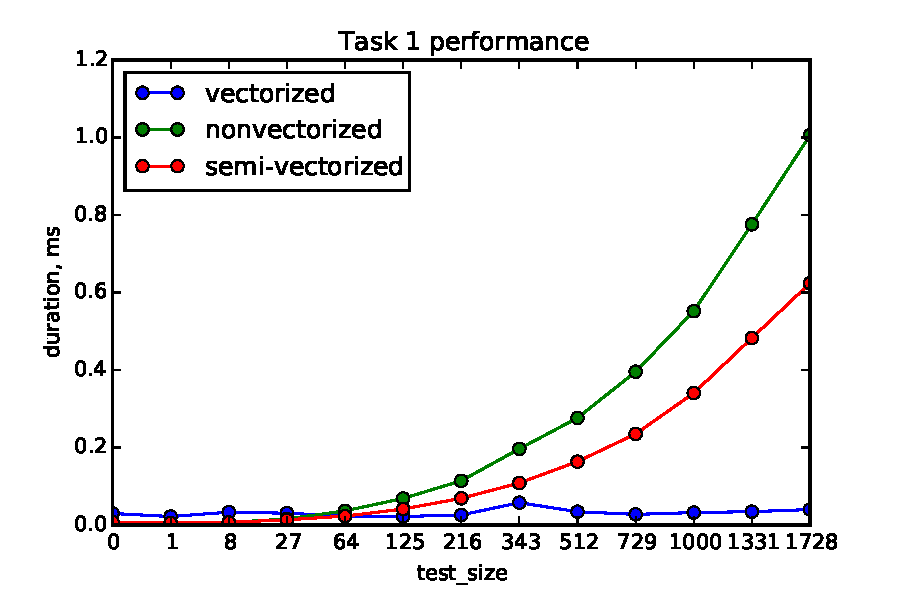
\includegraphics[scale=0.7]{task1}
	\end{center}
\end{figure}

\subsubsection*{Выводы}

Как видно, в целом, векторизованный вариант работает лучше двух других. Однако при небольших размерах данных имеет смысл использовать несложные алгоритмы. Видно, что при маленьких размерах обыкновенное умножение работает быстрее, чем np.prod.

\subsection{Задача 2}

\subsubsection*{Формулировка}

Даны матрица X и векторы одинаковой длины i и j. Построить вектор np.array(X[i[0], j[0]], \dots, X[i[N-1], j[N-1]]).

\newpage

\subsubsection*{Описание решений}

1. Векторизованный
\begin{lstlisting}
def new_vector1(X, i, j):
    return X[i, j]
\end{lstlisting}

2. В невекторизованном варианте заводится словарь, в который циклом добавляются элементы X[i[k], j[k]].

3. Заводится массив размера i.shape[0], в который циклом добавляются необходимые элементы.

\subsubsection*{Сравнение результатов}

\begin{figure}[h]
	\begin{center}
		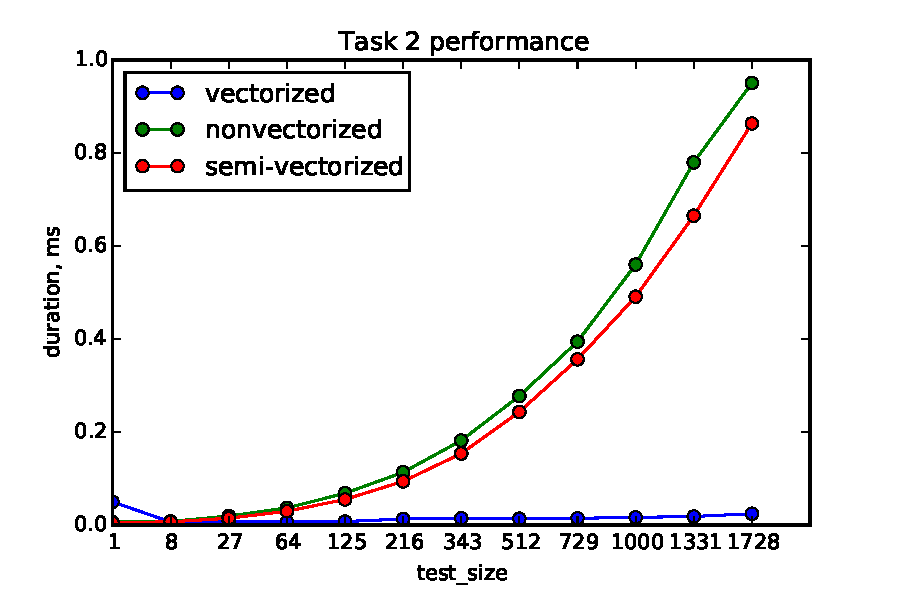
\includegraphics[scale=0.7]{task2}
	\end{center}
\end{figure}

\subsubsection*{Выводы}

Снова векторизованный вариант справляется быстрее с задачей почти на всех, даже небольших размерах выборки.

\subsection{Задача 3}

\subsubsection*{Формулировка}

Необходимо проверить, задают ли два вектора одинаковые мультимножества.

\subsubsection*{Описание решений}

1. Векторизованный
\begin{lstlisting}
def check_multisets1(x, y):
    return np.array_equal(np.sort(x), np.sort(y))
\end{lstlisting}

2. В невекторизованном варианте заводятся 2 словаря, содержащие все элементы векторов и их количество, а затем проверяется их равенство.

3. В третьем варианте векторы конвертируются в списки, которые, в свою очередь, сортируются и сравниваются.


\subsubsection*{Сравнение результатов}

\begin{figure}[h]
	\begin{center}
		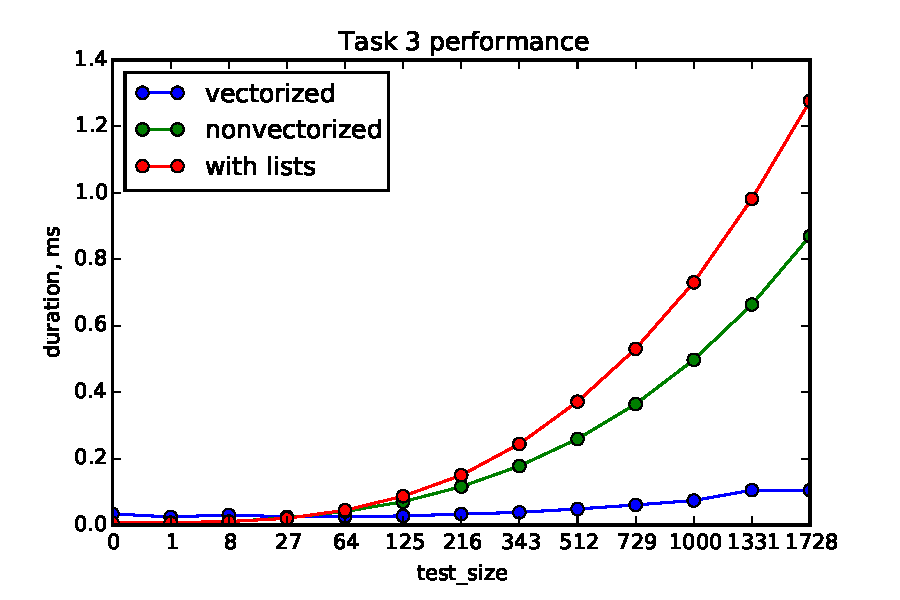
\includegraphics[scale=0.7]{task3}
	\end{center}
\end{figure}

\subsubsection*{Выводы}

В данной задаче (как, впрочем, и во многих других) векторизованный вариант --- самый простой и естественный, а другие --- лишь ненужное усложнение, поэтому и имеем такие результаты.

\subsection{Задача 4}

\subsubsection*{Формулировка}

В векторе найти максимальный элемент, следующий за нулевым.

\subsubsection*{Описание решений}

1. Векторизованный
\begin{lstlisting}
def max_after_zero1(x):
    return np.max(x[np.where(x[:-1:] == 0)[0] + 1])
\end{lstlisting}
Получаем набор индексов нулей, прибавляем 1, ищем максимум элементов с такими индексами.
В данном алгоритме сразу видно недостаток: при пустом x будет выдана ошибка. Но так как оговорено, что все объекты непустые (а также для того, чтобы код был в одну строку), такая проверка отсутствует.

2. Невекторизованный вариант: при нахождении нулевого элемента сравниваем с максимумом последующий элемент.

3. Заводится список всех элементов, следующих за нулем, и находится максимум.

\subsubsection*{Сравнение результатов}

\begin{figure}[h]
	\begin{center}
		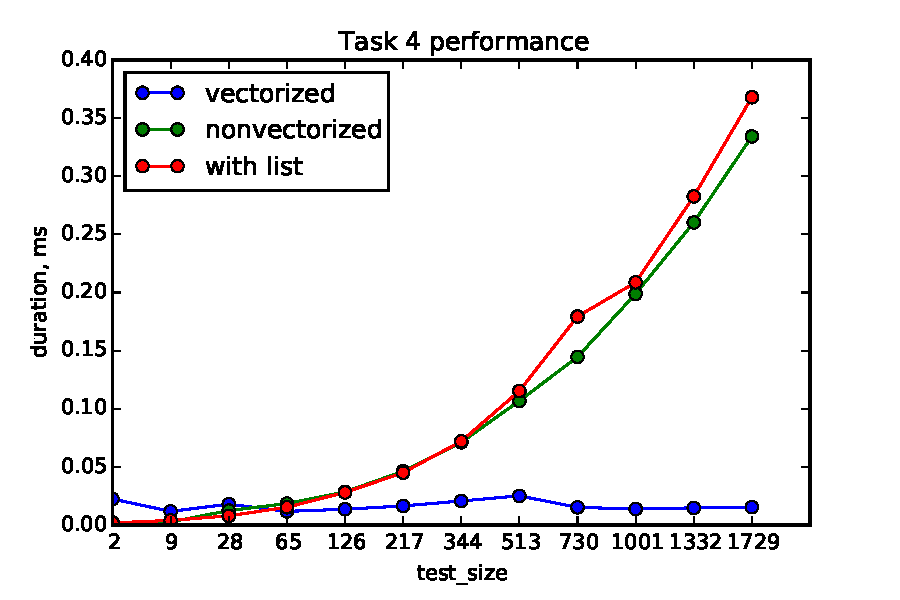
\includegraphics[scale=0.7]{task4}
	\end{center}
\end{figure}

\subsubsection*{Выводы}

Как видно, векторизованный вариант не слишком очевидный и не слишком простой, поэтому имеет смысл использовать простые модели на векторах длины меньше 50.

\subsection{Задача 5}

\subsubsection*{Формулировка}

Дан трёхмерный массив, содержащий изображение, размера (height, width, numChannels), а также вектор длины numChannels. Сложить каналы изображения с указанными весами, и вернуть результат в виде матрицы размера (height, width).

\subsubsection*{Описание решений}

1. Векторизованный
\begin{lstlisting}
def weighted_array_sum1(X, weights):
    return np.average(X, axis=2, weights=weights)
\end{lstlisting}

2. Невекторизованный --- тройной цикл по всему изображению и всем каналам.

3. Полувекторизованный --- цикл только по каналам.

\newpage

\subsubsection*{Сравнение результатов}

\begin{figure}[h]
	\begin{minipage}[h]{0.49\linewidth}
		\center{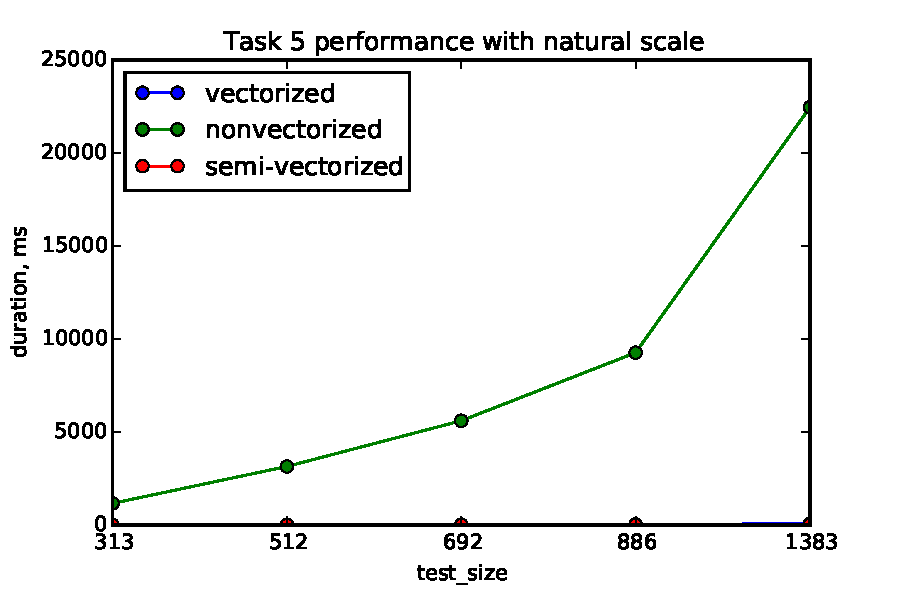
\includegraphics[width=\linewidth]{task5_2} \\ а)}
	\end{minipage}
	\hfill
	\begin{minipage}[h]{0.49\linewidth}
		\center{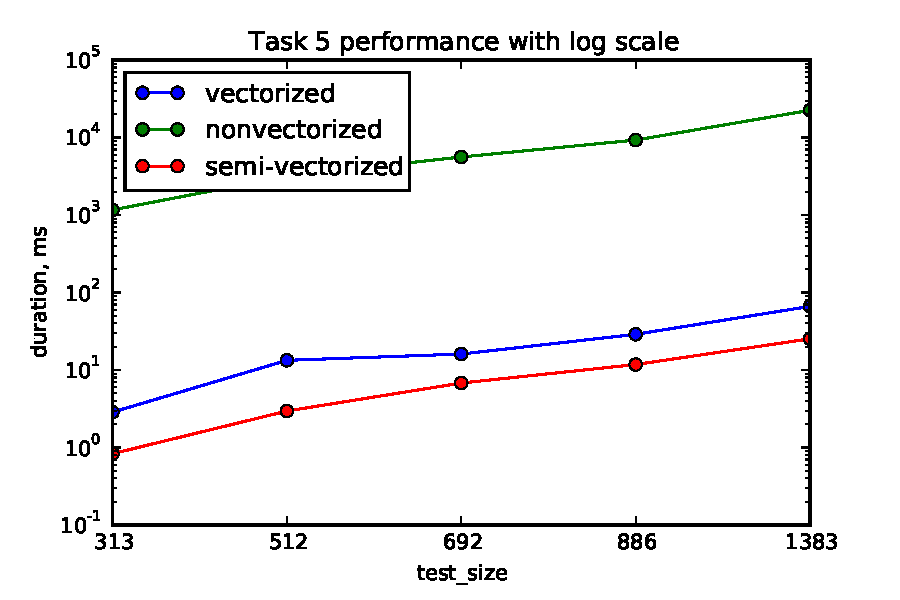
\includegraphics[width=\linewidth]{task5_1} \\ б)}
	\end{minipage}
	\caption{Зависимость времени работы алгоритмов в натуральной (линейной) и логарифмической шкале.}
\end{figure}

\subsubsection*{Выводы}

Полностью невекторизованный вариант работает чудовищно долго. В линейной шкале графики полу- и векторизованного варианта почти что совпадают с осью х. Однако заметно, что для 3-х каналов вариант алгоритма с циклом по всего лишь трем каналам работает хоть и не намного, но быстрее полностью векторизованного варианта.

\subsection{Задача 6}

\subsubsection*{Формулировка}

Необходимо реализовать Run-length encoding для произвольного вектора.

\subsubsection*{Описание решений}

1. Векторизованный вариант: находим индексы, в которых соседние элементы отличаются, вектор элементов с такими индексами плюс последний --- то, что ищем. Количество же определяется разницами между полученными индексами.

2. В невекторизованном варианте пробегаем по вектору, пока соседние элементы равны, увеличиваем счетчик на единицу, как только стали не равны, в список значений добавляем предыдущий элемент, а в количественный список текущее значение счетчика. Счетчик устанавливаем равным 1.

3. В третьем варианте "урезаются" последовательно равные элементы с добавлением в список их количества.

\newpage

\subsubsection*{Сравнение результатов}

\begin{figure}[h]
	\begin{center}
		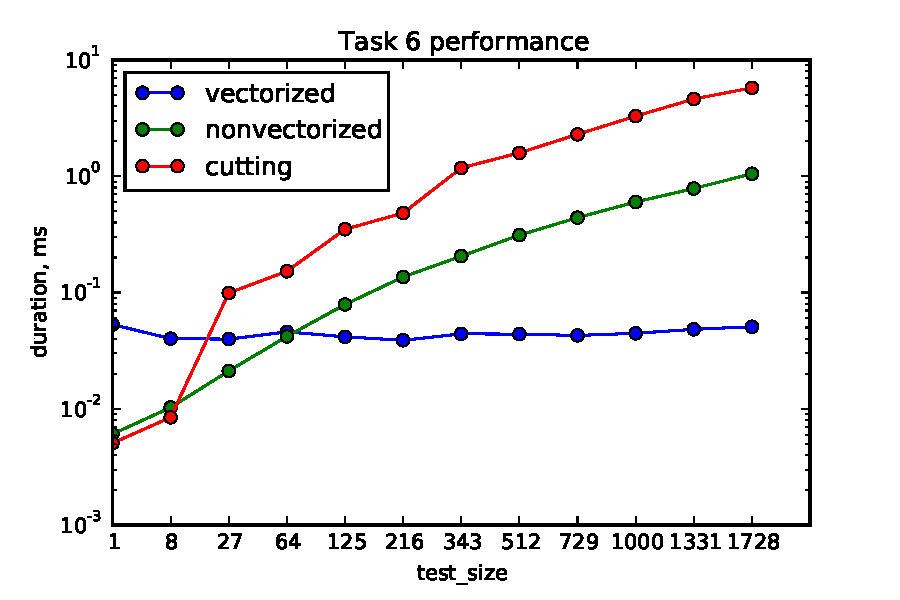
\includegraphics[scale=0.7]{task6}
	\end{center}
\end{figure}

\subsubsection*{Выводы}

Все алгоритмы достаточно сложные, но, как всегда, асимптотически побеждает векторизованный вариант.

\subsection{Задача 7}

\subsubsection*{Формулировка}

Даны две выборки объектов - X и Y. Вычислить матрицу евклидовых расстояний между объектами. Сравнить с SciPy реализацией.

\subsubsection*{Описание решений}

1. Векторизованный (с использованием broadcasting)
\begin{lstlisting}
def object_dist1(X, Y):
    return np.sqrt(np.sum((X[:, :, np.newaxis] - 
    Y.T[np.newaxis, :, :]) ** 2, axis=1))
\end{lstlisting}

2. Тройной цикл

3. Третий вариант --- полувекторизованный, тоже с использованием broadcasting. Находятся расстояния между всей матрицей Х и отдельной строкой Y. При этом в результирующую матрицу ответы записываются построчно.

\newpage

\subsubsection*{Сравнение результатов}

\begin{figure}[h]
	\begin{center}
		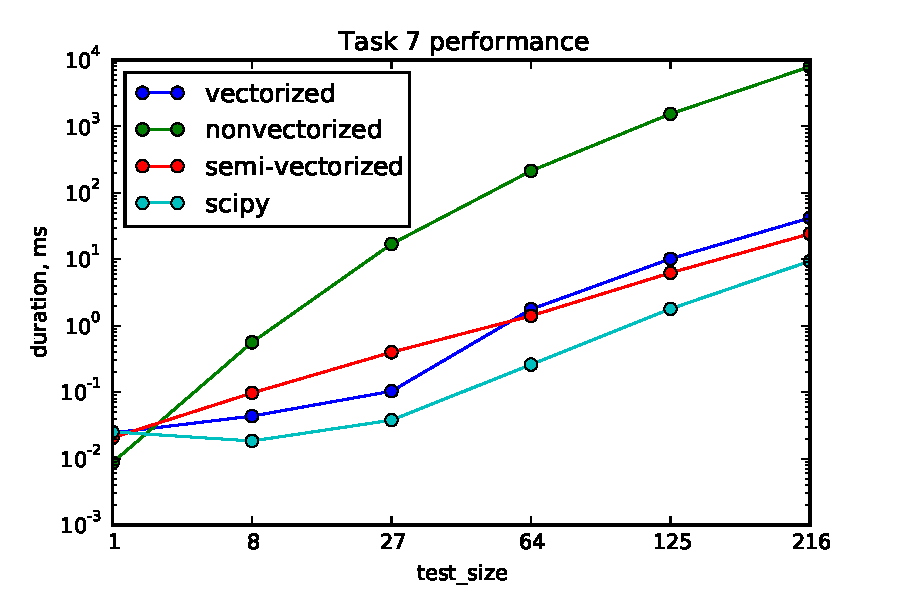
\includegraphics[scale=0.7]{task7}
	\end{center}
\end{figure}

\subsubsection*{Выводы}
С циклами выходит все колоссально долго (обратите внимание на логарифмическую шкалу). Остальные же реализации работают примерно одинаково, но готовая реализация все же чуточку лучше.

\subsection{Задача 8}

\subsubsection*{Формулировка}

Реализовать функцию вычисления логарифма плотности многомерного нормального распределения. Входные параметры: точки X, размер (N, D), мат. ожидание m, вектор длины D, матрица ковариаций C, размер (D, D).
Плотность многомерного нормального распределения имеет формулу:
\[
	f(\bold{x}) = \frac{1}{(2\pi)^{n/2}|C|^{1/2}}e^{-\frac{1}{2}(\bold{x}-m)C^{-1}(\bold{x}-m)^T}
\]

\subsubsection*{Описание решений}

1. Векторизованный
\begin{lstlisting}
def function1(X, m, C):
    return np.diag(np.log(np.exp(-0.5 * np.dot(np.dot((X-m),
    np.linalg.inv(C)), (X-m).T)) / ((2*np.pi) ** 
    (X.shape[1]/2.0) * (np.linalg.det(C))**0.5)))
\end{lstlisting}

2. Делается всё то же самое, только все векторные вычисления (кроме подсчета обратной матрицы ковариации и ее определителя) заменены на вычисления через циклы.

3. Полувекторизованный --- невекторизованный вариант с векторными вычислениями произведений матриц.

\subsubsection*{Сравнение результатов}

\begin{figure}[h]
	\begin{center}
		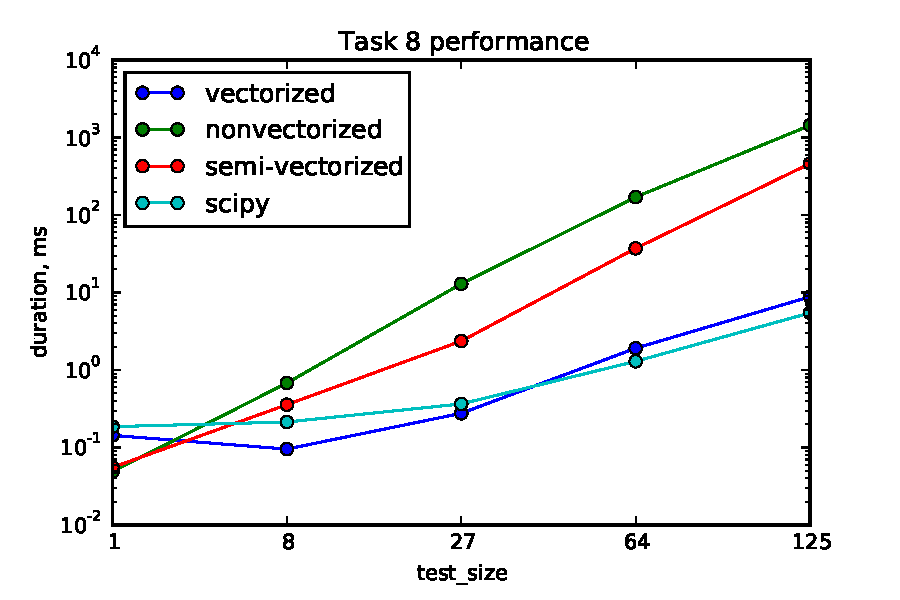
\includegraphics[scale=0.7]{task8}
	\end{center}
\end{figure}

\subsubsection*{Выводы}
Как и ожидалось, векторизованный вариант лучше всех, содержащих невекторизованные операции, но чуть хуже встроенной реализации.

\section{Глобальные выводы}
Как можно заметить, в серьезных задачах следует использовать векторизацию всегда, когда возможно (по крайней мере, судя по данным задачам). Это объясняется тем фактом, что циклы в языке Python работают значительно дольше, чем циклы в языке C++, на котором реализовано ядро NumPy и Scipy. Однако если гарантировано, что функция будет работать с данными небольших размеров, имеет смысл задуматься над простой, быстрой по написанию реализацией. Также написание невекторизованных функций полезно для демонстрации быстроты работы векторизованных вариантов.

\end{document}
